\documentclass{beamer}

% Packages
% ---
%\usepackage{amsmath} % Advanced math typesetting
\usepackage[utf8]{inputenc} % Unicode support (Umlauts etc.)
\usepackage[italian]{babel} % Change hyphenation rules
\usepackage{hyperref} % Add a link to your document
\usepackage{graphicx} % Add pictures to your document
\usepackage[export]{adjustbox}
\usepackage{listings} % Source code formatting and highlighting
\usepackage{caption}
\usepackage{subcaption}

\graphicspath{ {./img/} }

\newcommand{\quotes}[1]{``#1''}

%Information to be included in the title page:
\title{DataVirus.it}
\author{Federico Rachelli}
\institute{Alma Mater Studiorum - Universitá di Bologna}
\date{19/06/2020}

\begin{document}
    \frame{\titlepage}
    
    \begin{frame}
        \frametitle{Introduzione}
        DataVirus.it é una applicazione per piattaforma Android ispirata al \href{https://datavirus.it}{sito web omonimo}.
        Dall'app si possono vedere gli ultimi aggiornamenti sull'epidemia di COVID-19 in Italia in modo facile ed intuitivo.
        \\
        L'app ottiene i dati provenienti dal Dipartimento di Protezione Civile e li elabora, rendendoli di facile visione ed interazione, servendosi ulteriormente della costruzione di grafici \emph{real-time} per l'evoluzione della malattia nel tempo.
    \end{frame}

    \begin{frame}
        \frametitle{Schermata principale - MainActivity}
        \noindent\begin{minipage}{0.3\textwidth}% adapt widths of minipages to your needs
            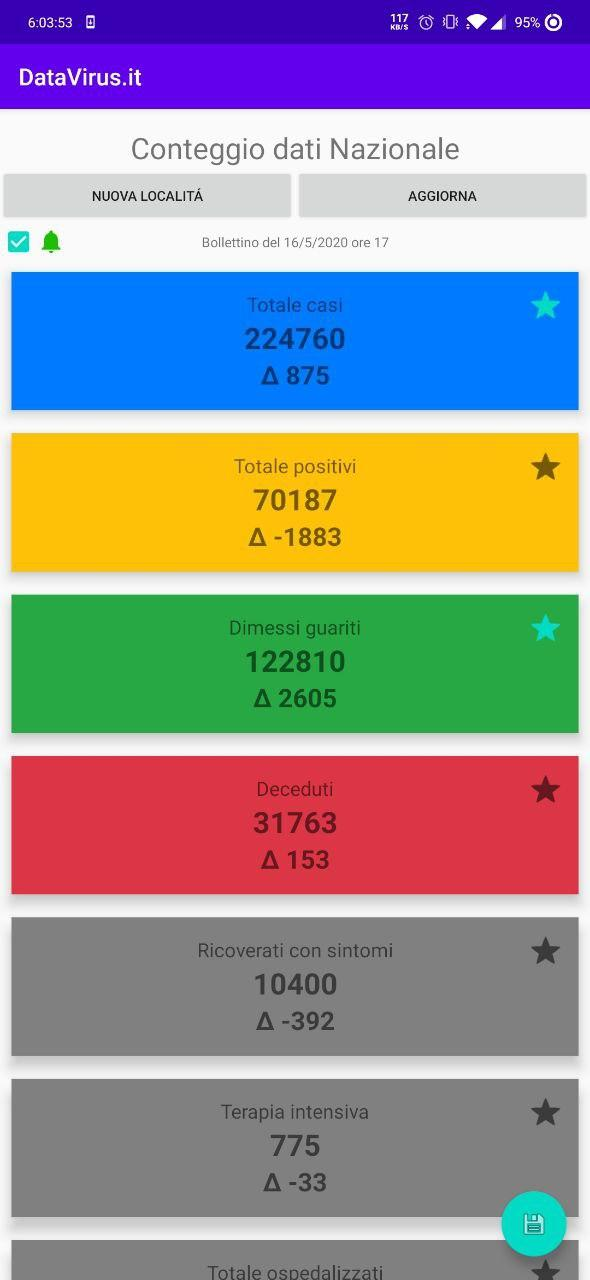
\includegraphics[width=\linewidth]{main_activity.jpg}
        \end{minipage}%
        \hfill%
        \begin{minipage}{0.6\textwidth}\raggedleft
            All'apertura dell'app verranno scaricati i dati aggiornati dal
            \href{https://github.com/pcm-dpc/COVID-19}{GitHub repository ufficiale} del Dipartimento di Protezione Civile
            e verrá mostrato l'andamento dell'epidemia attraverso tiles contenenti i dati e il loro incremento (delta) rispetto alla giornata precedente.
            \\
            Nella parte alta dell'activity viene mostrato l'ambito geografico (alla prima apertura verrá sempre mostrato l'andamento nazionale),
            e di seguito i pulsanti \quotes{Aggiorna} e \quotes{Nuova localitá} assieme alla data/ora in cui i dati sono stati aggiornati dal DPC.
            \\
            
        \end{minipage}
    \end{frame}

    \begin{frame}
        \frametitle{Cambio zona geografica - GeoPicker}
        \noindent\begin{minipage}{0.3\textwidth}% adapt widths of minipages to your needs
            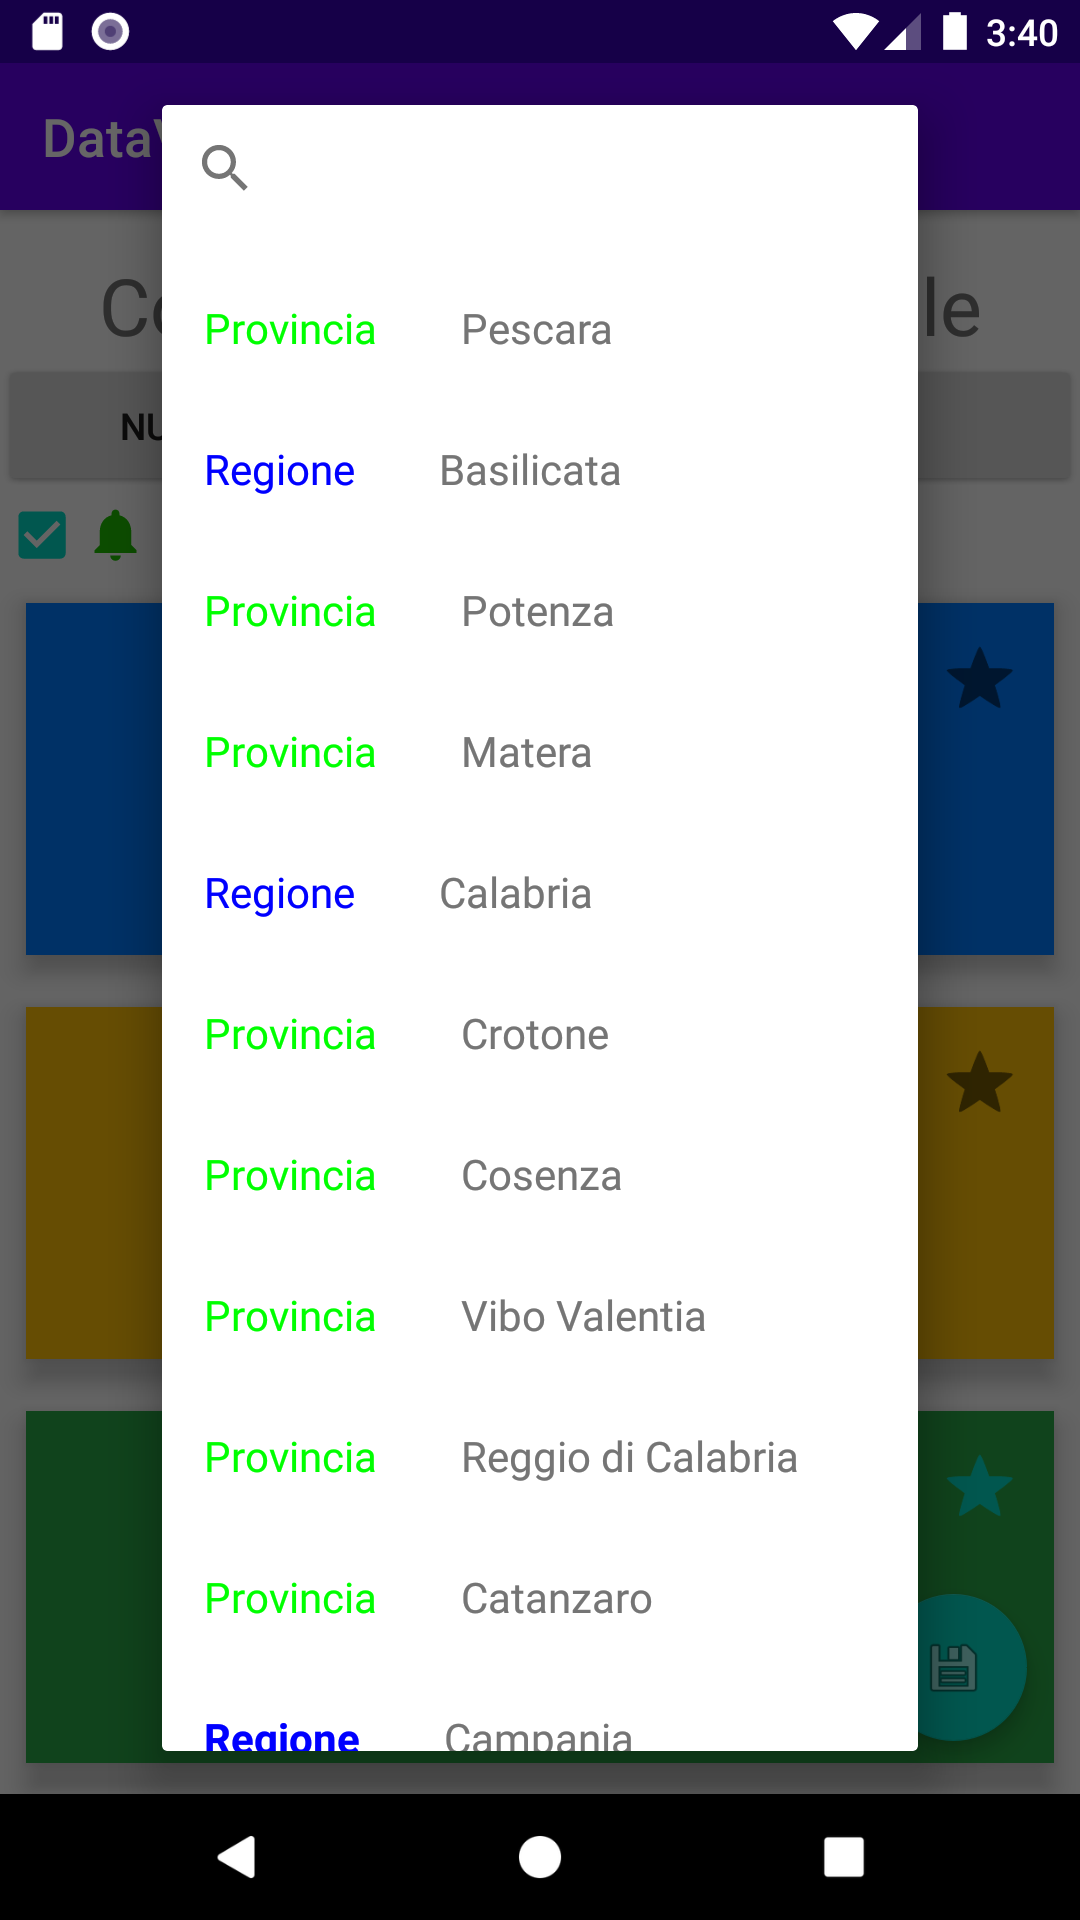
\includegraphics[width=\linewidth]{DPC_geo_picker.png}
        \end{minipage}%
        \hfill%
        \begin{minipage}{0.6\textwidth}\raggedright
            Quando si preme sul pulsante \quotes{Nuova localitá} si aprirá un dialog dove si potrá scegliere la regione o provincia d'interesse.
            Si potrá anche scegliere di visionare nuovamente il dato nazionale (in prima posizione).
            \\
            Una volta premuto sul nome della zona d'interesse, si verrá rediretti nuovamente sulla MainActivity e verrá mostrato l'andamento per la regione/procvincia d'interesse.
        \end{minipage}
    \end{frame}

    \begin{frame}
        \frametitle{Cambio zona geografica - MainActivity}
        \noindent\begin{minipage}{0.3\textwidth}% adapt widths of minipages to your needs
            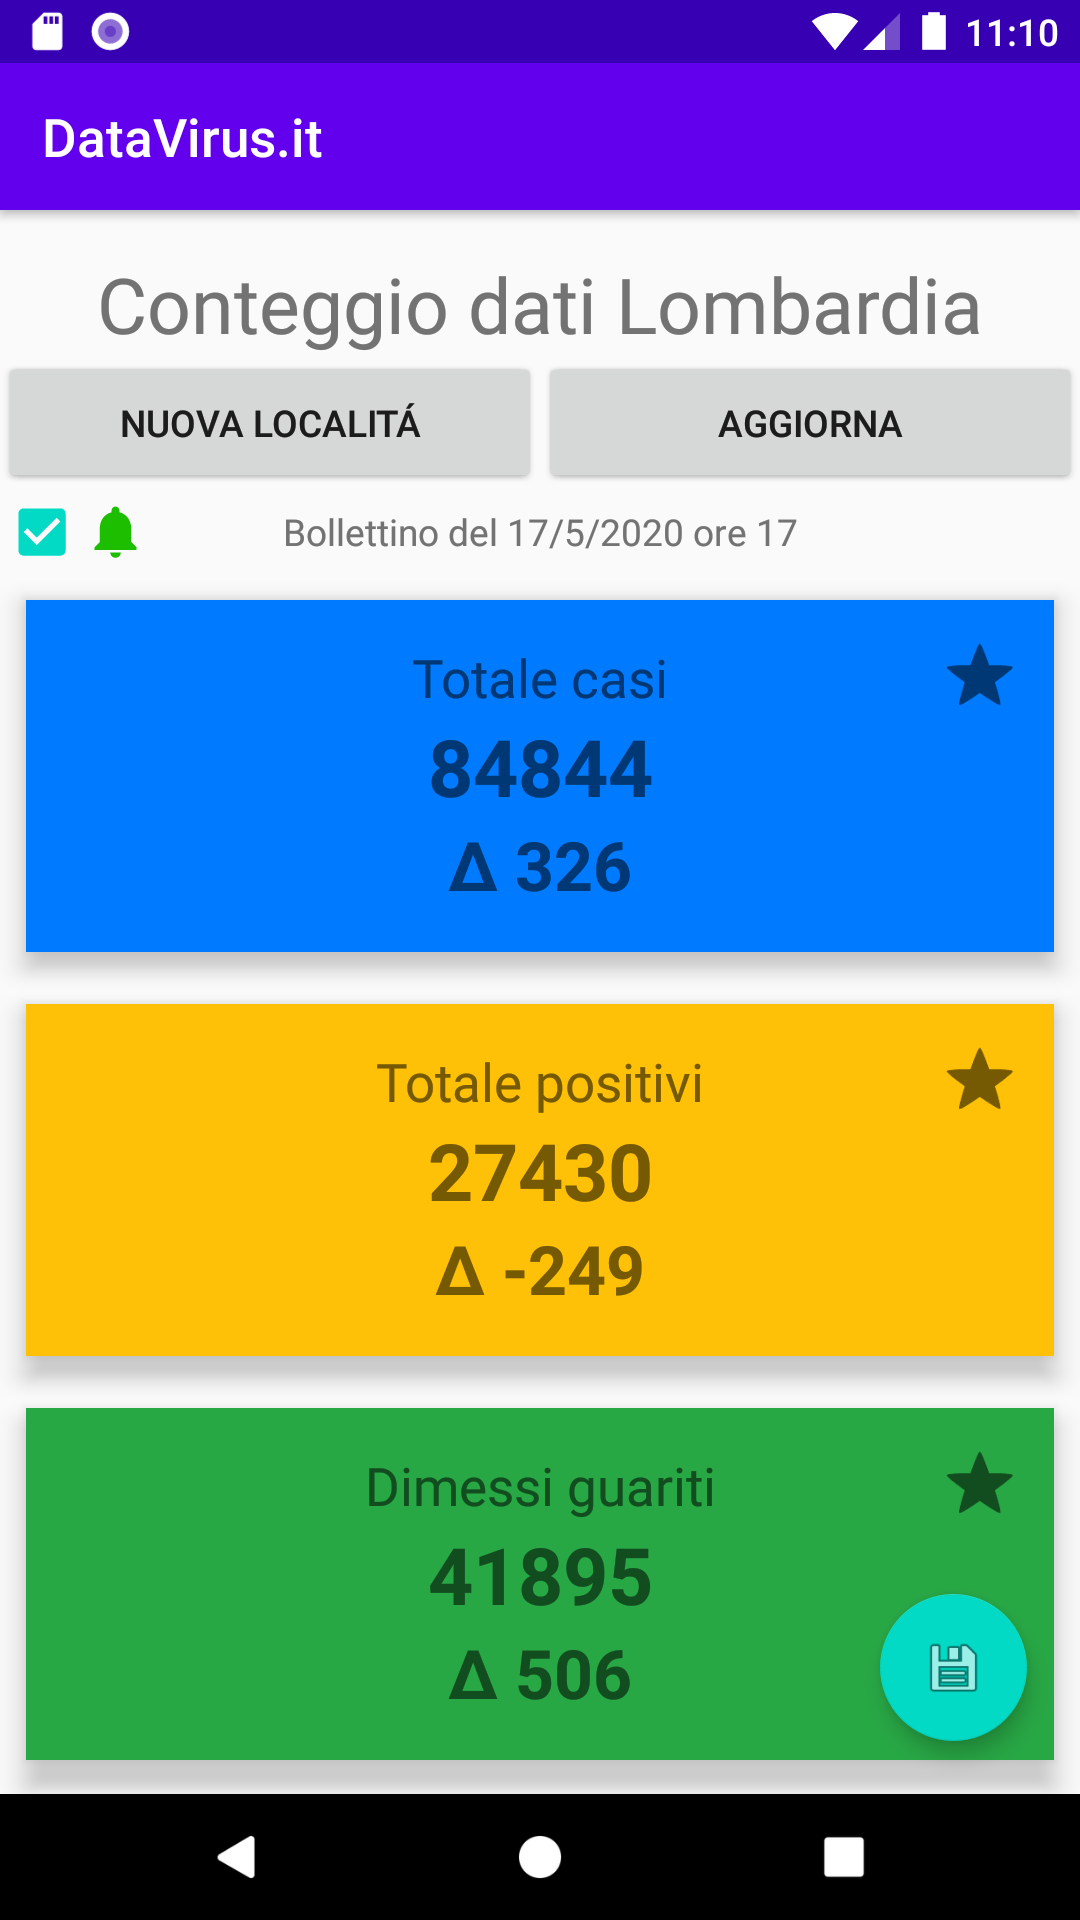
\includegraphics[width=\linewidth]{lombardia.png}
        \end{minipage}%
        \hfill%
        \begin{minipage}{0.6\textwidth}\raggedright
            Nell'immagine viene mostrato un'andamento regionale (in particolare della regione Lombardia).
            \\
            \emph{Nota:} per gli andamenti provinciali il Dipartimento di Protezione Civile raccoglie solamente il dato relativo al totale dei casi.
        \end{minipage}
    \end{frame}

    \begin{frame}
        \frametitle{Grafici - ChartActivity (1/2)}
        \noindent\begin{minipage}{0.3\textwidth}% adapt widths of minipages to your needs
            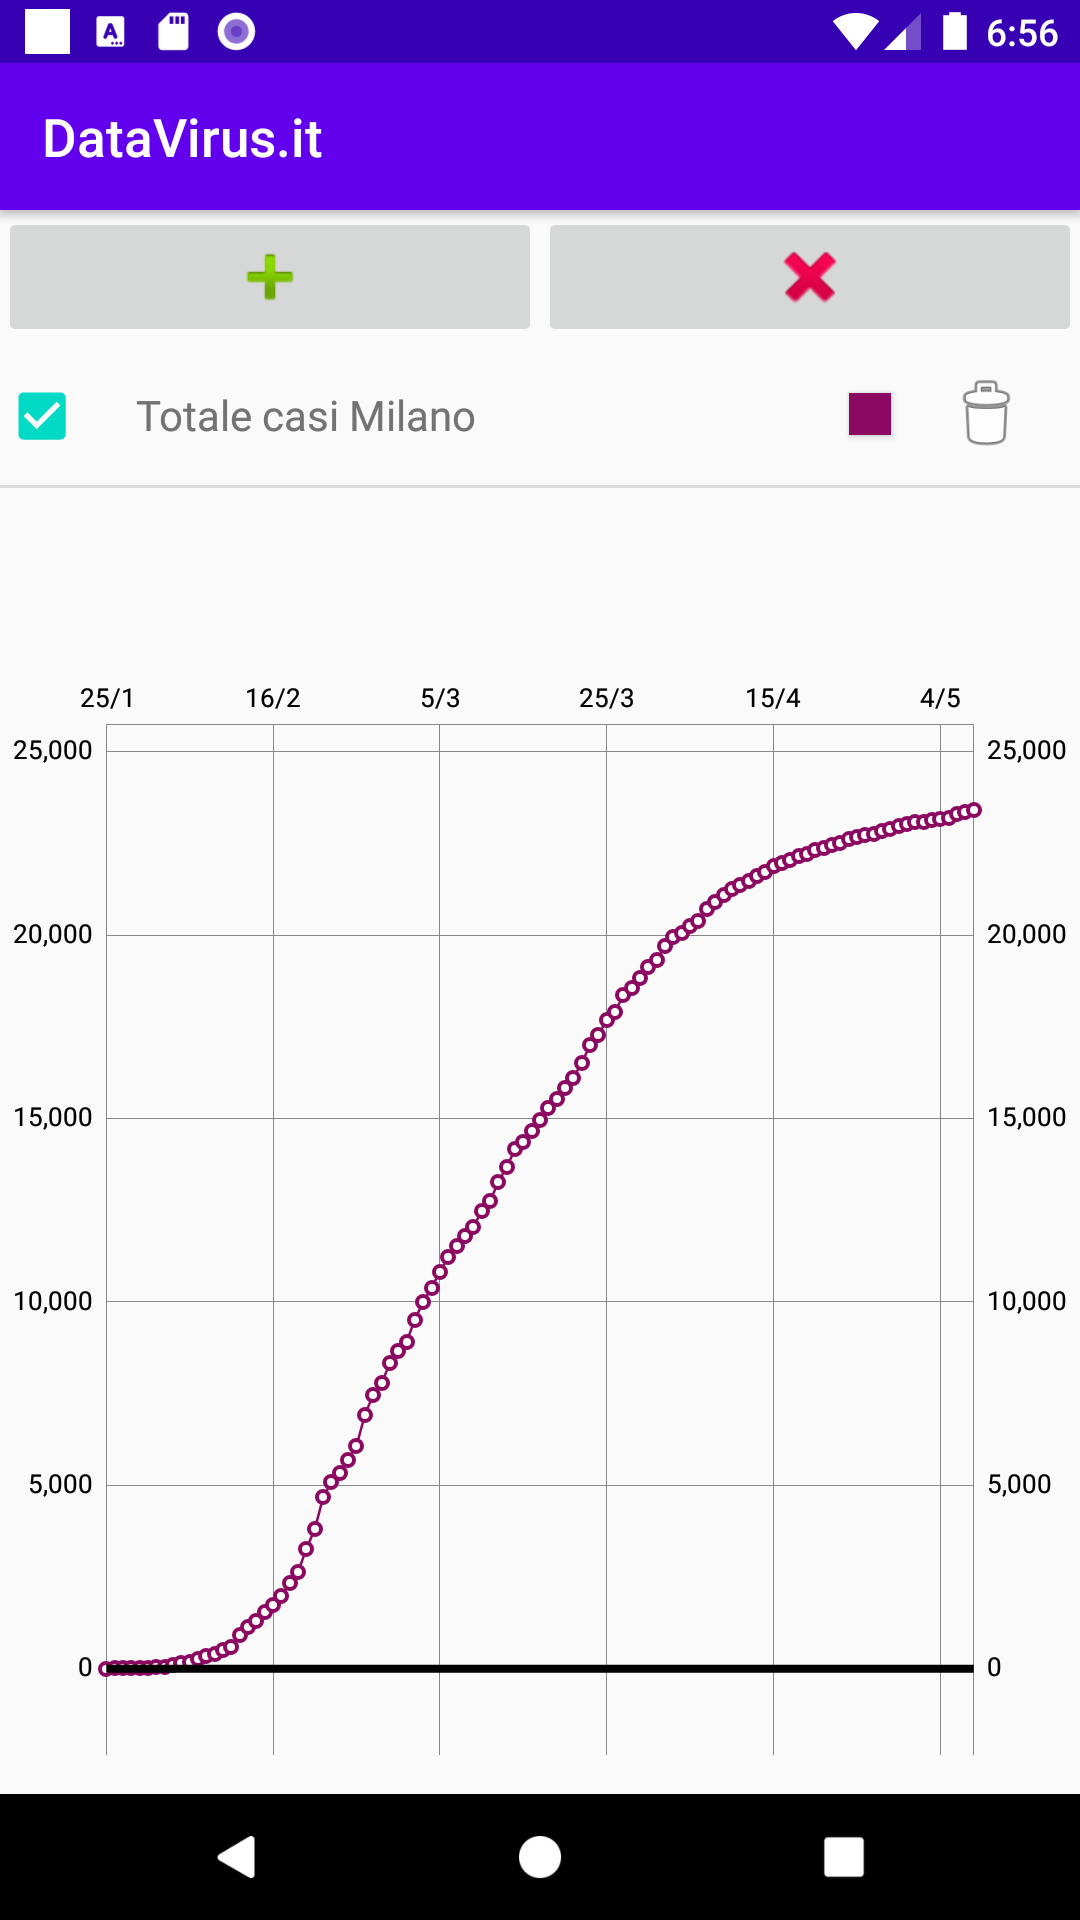
\includegraphics[width=\linewidth]{milano.png}
        \end{minipage}%
        \hfill%
        \begin{minipage}{0.6\textwidth}\raggedright
            Se si preme su una tile, verrá mostrato il grafico dell'andamento nel tempo di tale dato.
            \\
            Il grafico si puó ingrandire a piacimento tramite il \emph{pinch-to-zoom}. 
            Zoomando verranno mostrati i dati della singola giornata.
            \\
            A fianco un'esempio di un grafico con il solo dato dei positivi della provincia di Milano.
        \end{minipage}
    \end{frame}

    \begin{frame}
        \frametitle{Grafici - ChartActivity (2/2)}
        \noindent\begin{minipage}{0.3\textwidth}% adapt widths of minipages to your needs
            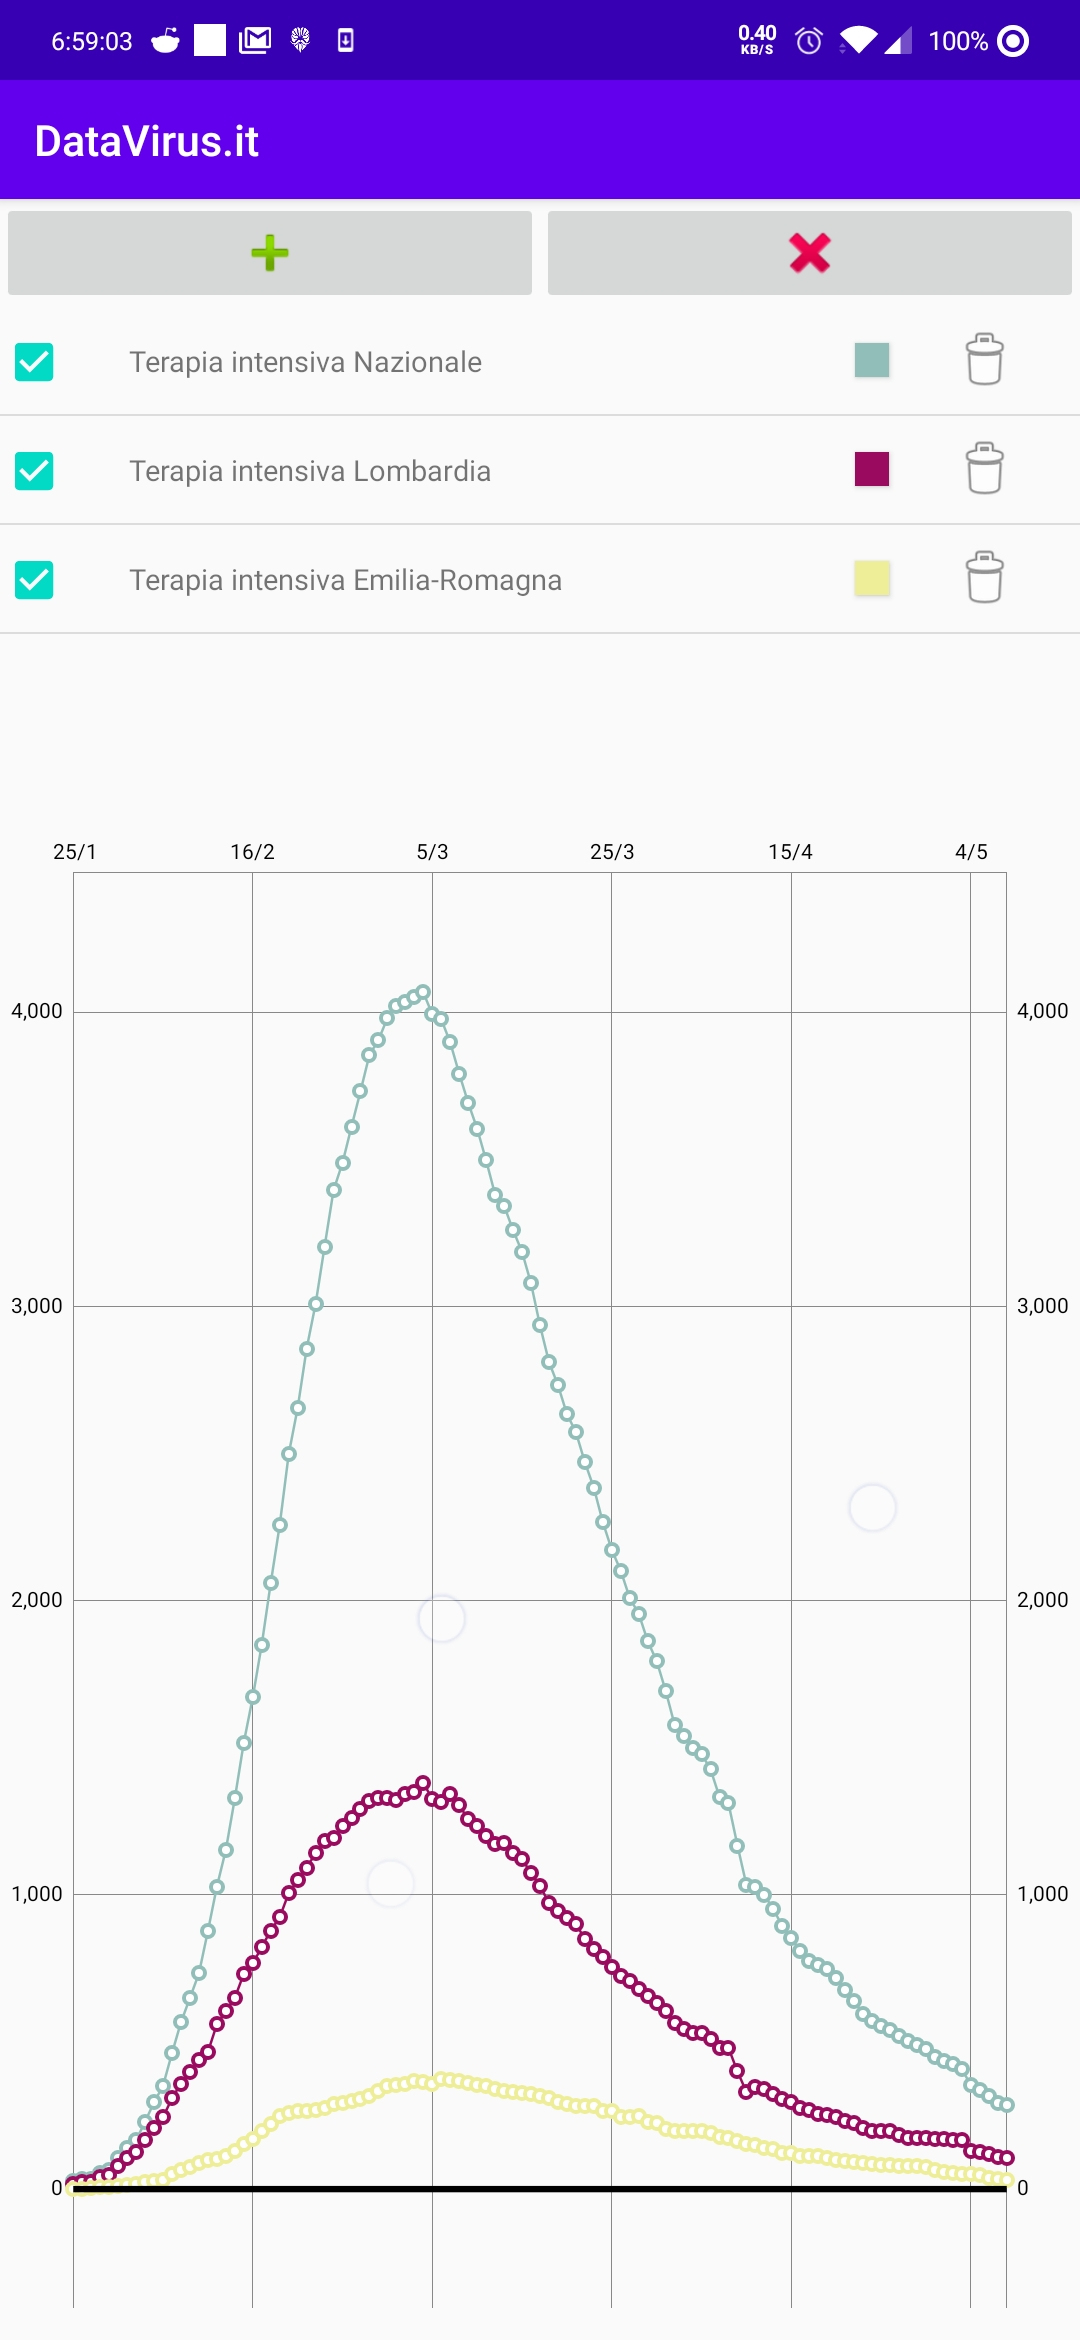
\includegraphics[width=\linewidth]{chart_ICU.jpg}
        \end{minipage}%
        \hfill%
        \begin{minipage}{0.6\textwidth}\raggedright
            Si possono aggiungere dati ulteriori per costruire grafici piú complessi. Il pulsante \quotes{+} permette di scegliere un'ulteriore dato da aggiungere al grafico.
            \\
            Premento la \quotes{X} si cancelleranno tutti i dati finora inseriti, resettando il grafico.
            \\
            Il pulsante con il \emph{cestino} cancella il singolo dato.
            \\
            A fianco un'esempio di un grafico che paragona i posti occupati in terapia intensiva, mostrando nel tempo il dato nazionale e quello delle regioni Lombardia ed Emilia-Romagna.
        \end{minipage}
    \end{frame}

    \begin{frame}
        \frametitle{Preferiti - StarredActivity}
        \noindent\begin{minipage}{0.3\textwidth}% adapt widths of minipages to your needs
            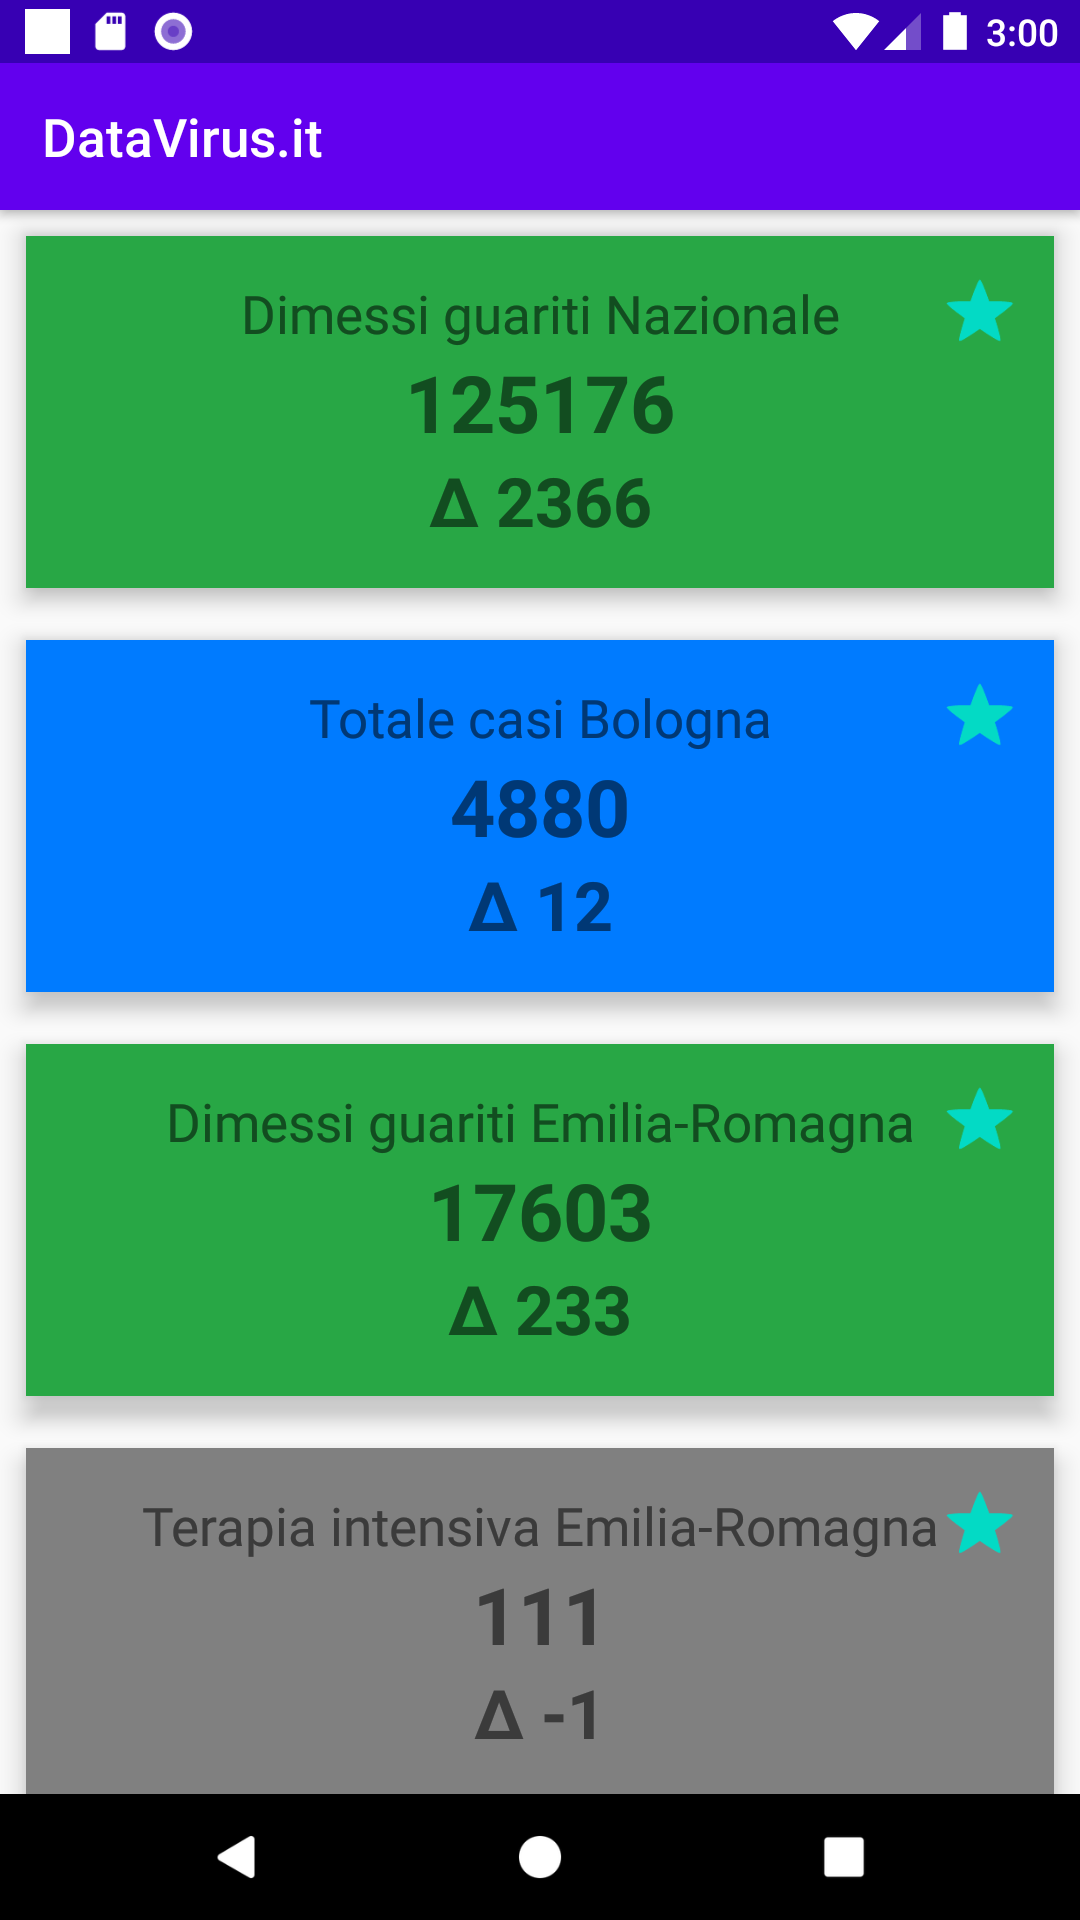
\includegraphics[width=\linewidth]{preferences.png}
        \end{minipage}%
        \hfill%
        \begin{minipage}{0.6\textwidth}\raggedright
            Dalla \emph{MainActivity}, premendo sul \emph{Floating Action Button} (in basso a destra) si potranno visionare i dati marcati come \emph{starred}.
            \\
            Per inserire/rimuovere dai preferiti un dato é sufficiente premere sulla \emph{stellina} in alto a destra presente in ogni tile.
        \end{minipage}
    \end{frame}

    \begin{frame}
        \frametitle{Notifiche periodiche - DataNotifyReceiver}
        
\includegraphics[width=\linewidth]{notif.jpg}
        Il Dipartimento di Protezione Civile aggiorna quotidianamente i dati dalle h.18:00 in poi.
        Da quell'orario l'app esegue in background una ricerca (a cadenza di 10 minuti) della disponibilitá dei dati.
        \\
        Nel caso siano disponibili verrá notificato all'utente. Alla pressione della notifica verrá aperta l'app.
        \\
        Le notifiche periodiche possono essere attivate o disattivate tramite la checkbox in alto a sinistra nella \emph{MainActivity}.
    \end{frame}

\end{document}